% STATUS: ACTIVE -- 2026-10-19 (user): block diagram of the regulation of the motion gain, built on the motion control loop of
%   TIE 2025 Fig. 2 (inner loop, kept as in the paper) with the outer regulation loop of Meng 2023 dissertation Fig. 44 / (6.17)-(6.19).
%   Colors from the Interview Slides design system (paper, panel, line, ink, ink-muted, signal, copper); math in Times (newtx), as its
%   equations.md asks. Compile: pdflatex fig_1019_regulation_block.tex (in figures/src), then pdftoppm -r 300 -png for the slide.
\documentclass[border=0pt]{standalone}
\usepackage{newtxtext,newtxmath}
\usepackage{tikz}
\usetikzlibrary{arrows.meta,calc,fit,backgrounds}
\definecolor{paper}{HTML}{F4F6F7}
\definecolor{panel}{HTML}{E6ECEF}
\definecolor{line}{HTML}{B9C4CB}
\definecolor{ink}{HTML}{15222C}
\definecolor{inkmuted}{HTML}{4E5D68}
\definecolor{signal}{HTML}{14607F}
\definecolor{signalsoft}{HTML}{D5E7EE}
\definecolor{copper}{HTML}{9A4A20}
\definecolor{coppersoft}{HTML}{F3E0D3}
\begin{document}
\begin{tikzpicture}[
  font=\small, >={Triangle[length=5pt,width=4pt]},
  blk/.style={draw=ink, line width=0.6pt, rounded corners=1.5pt, fill=paper, minimum height=11mm, align=center, inner sep=4pt},
  reg/.style={blk, draw=signal, fill=signalsoft},
  lim/.style={blk, draw=copper, fill=coppersoft, line width=1.2pt},
  sum/.style={draw=ink, line width=0.6pt, circle, minimum size=5mm, inner sep=0pt, fill=paper},
  ink arrow/.style={->, line width=0.7pt, draw=ink},
  sig arrow/.style={->, line width=1.1pt, draw=signal},
  lab/.style={font=\small, text=ink},
  slab/.style={font=\small, text=signal},
  note/.style={font=\small\itshape, text=inkmuted},
]
% ---------------- blocks ----------------
\node[sum] (s) at (0,0) {};
\node[reg, minimum width=30mm] (rg) at (2.7,0) {Regulator\\[2pt]$(1-\lambda_a)\,\dfrac{\bar{a}_d-\hat{\bar{a}}}{\hat{\bar{a}}'}$};
\node[lim, minimum width=22mm] (lm) at (6.3,0) {Limit\\[1pt]$|\Delta\bar{x}_d| \le v_{\max}$};
\node[blk, draw=signal, minimum width=15mm] (acc) at (9.0,0) {$\dfrac{1}{1-z^{-1}}$};
\node[blk, minimum width=24mm] (law) at (11.9,0) {Motion\\control law};
\node[blk, minimum width=24mm] (force) at (15.0,0) {Magnetic force\\generation};
\node[blk, minimum width=24mm] (dyn) at (18.1,0) {Particle\\dynamics};
\node[blk, minimum width=24mm] (track) at (18.1,-2.5) {Visual tracking\\$z^{-2}$};
\node[blk, minimum width=34mm] (est) at (13.4,-2.5) {Estimator\\$\delta\hat{\bar{x}}_{1,2,3},\ \hat{\bar{a}},\ \hat{\bar{a}}'\ \text{or}\ \hat{\bar{w}}_s$};
\node[blk, draw=signal, minimum width=22mm] (slope) at (2.3,-4.3) {$\hat{\bar{a}}' = 1/\hat{h}^{2}$};

% ---------------- backgrounds ----------------
\begin{scope}[on background layer]
  \node[fit=(law)(force)(dyn)(track)(est), inner xsep=6mm, inner ysep=7mm, fill=panel, draw=line, line width=0.6pt, dashed] (mc) {};
  \fill[paper] ($(current bounding box.south west)+(-12mm,-14mm)$) rectangle ($(current bounding box.north east)+(8mm,10mm)$);
  \node[fit=(law)(force)(dyn)(track)(est), inner xsep=6mm, inner ysep=7mm, fill=panel, draw=line, line width=0.6pt, dashed] {};
\end{scope}
\node[note, anchor=north west] at ($(mc.north west)+(1.5mm,-1mm)$) {motion control};

% ---------------- motion control loop (TIE 2025 Fig. 2) ----------------
\draw[ink arrow] (law) -- node[above, lab] {$\bar{f}_d$} (force);
\draw[ink arrow] (force) -- node[above, lab] {$\bar{f}_m$} (dyn);
\draw[ink arrow] (dyn.east) -- ++(5mm,0) node[above, lab] {$\bar{x}$} |- (track.east);
\draw[ink arrow] (track) -- node[above, lab] {$\delta\bar{x}_m$} (est);
\draw[ink arrow] (est.north -| law.south) -- node[left, lab] {$\delta\hat{\bar{x}}_3,\ \hat{\bar{a}}$} (law.south);

% ---------------- regulation loop ----------------
\node[lab, anchor=east] (ad) at (-0.9,0) {$\bar{a}_d$};
\draw[sig arrow] (ad) -- (s);
\node[font=\scriptsize, text=ink] at (-0.42,0.32) {$+$};
\node[font=\scriptsize, text=ink] at (0.36,-0.36) {$-$};
\draw[sig arrow] (s) -- (rg);
\draw[sig arrow] (rg) -- (lm);
\draw[sig arrow] (lm) -- node[above, slab] {$\Delta\bar{x}_d$} (acc);
\draw[sig arrow] (acc) -- node[pos=0.35, above, slab] {$\bar{x}_d$} (law);
\node[font=\small\itshape, text=copper, anchor=south] at ($(lm.north)+(0,1mm)$) {$\bar{a}'$ as a state variable only};

% estimates back to the regulator: three ports under the estimator
\coordinate (pA) at ($(est.south)+(-1.4,0)$);   % a-hat' (slope as a state variable)
\coordinate (pW) at ($(est.south)+(0,0)$);      % w_s-hat (wall position as a state variable)
\coordinate (pa) at ($(est.south)+(1.4,0)$);    % a-hat
\draw[sig arrow] (pa) -- ++(0,-2.9) -| node[pos=0.25, above, slab] {$\hat{\bar{a}}$} (s.south);
\draw[sig arrow] (pW) |- node[pos=0.75, below, slab] {$\hat{\bar{w}}_s$} (slope.east);
\draw[sig arrow] (slope.north) -- node[left, slab] {$\hat{\bar{a}}'$} ($(rg.south)+(-0.4,0)$);
\draw[sig arrow, dashed] (pA) -- ++(0,-0.9) -| node[pos=0.3, above, slab] {$\hat{\bar{a}}'$\ \ \textit{($\bar{a}'$ as a state variable)}} ($(rg.south)+(0.6,0)$);

\node[note, anchor=north] at ($(slope.south)+(0,-1mm)$) {$\bar{w}_s$ as a state variable};
\end{tikzpicture}
\end{document}
